\documentclass[10pt]{beamer}

\usepackage[utf8]{inputenc}
\usepackage{pgfpages}
\usepackage{dirtree}
\setbeamertemplate{note page}[plain]
\AtEndNote{\vfill \begin{center} mm:hh \end{center}}
\newcommand{\notedir}[1] {
  \note{\dirtree{#1}}}
\usepackage{tcolorbox}
\usepackage{tikz}
\usetikzlibrary{intersections,calc}
\usepackage{amsmath}
\usepackage{graphicx}
\def \heart {\textcolor{blue}{$\heartsuit$} }
\def \C {$\mathcal{C}$}





\tcbset{%
	basic/.style={colframe=black,
		      colback=white,
		      top= 0mm,
		      bottom = 2mm,
		      boxsep=0mm
		      }
}

    
\begin{document}  
    \setlength{\abovedisplayskip}{0pt}
    \setlength{\belowdisplayskip}{0pt}
    
    \beamertemplatenavigationsymbolsempty
    
    \frame{
	   \frametitle{Q1 Juillet 2015.}

	    Un point $P$ appartient à la diagonale $BD$ d'un carré $ABCD$. On note $c$ la longueur de chacun des côtés de ce carré. 
	    Démontrer l'égalité $$\overrightarrow{BP} \cdot \overrightarrow{DP} = ||\overrightarrow{AP}||^2 - c^2.$$

	    \vfill
	  
	  \pause
	  % hypothèses et thèse
	  \begin{tcolorbox}[basic] 
	      \begin{columns}[t]
		 
		 \column{.5\textwidth}\centering
		      
		      \underline{Hypothèses} 
		      \begin{itemize}
		      \item $ABCD$ carré.
		      \end{itemize}

		  
		  \column{.5\textwidth}\centering
		      
		      \underline{Thèse} \\
		      \smallskip
		      $\overrightarrow{BP} \cdot \overrightarrow{DP} = ||\overrightarrow{AP}||^2 - c^2.$
		
	      \end{columns}
	  \end{tcolorbox}
    
    
	   \notedir{%
	   .1 Énoncé.
	   .2 Choix : Géométrique synthétique.
	   .3 Égalité de longueurs et présence de triangles..
	   .4 Hypothèses (non visibles sur le dessin)..
	   .4 Thèse..
	   .4 Grand dessin..
	   }
	   }

	   
 \frame{ % résolution ex1
	  \begin{columns}[t]
		\column{.5\textwidth}\centering 
		

			\underline{Dessin}\\
			
				  \begin{figure}[h]
				  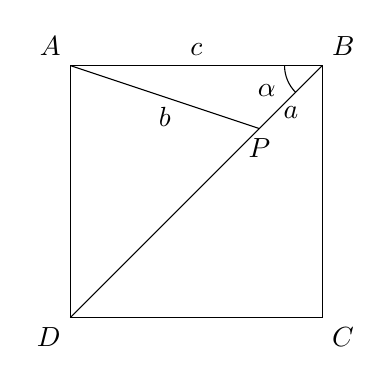
\begin{tikzpicture}[scale=0.8]
					\coordinate[label=above left:$A$] (A) at (-2,2);
					\coordinate[label=above right:$B$] (B) at (2,2);
					\coordinate[label=below right:$C$] (C) at (2,-2);
					\coordinate[label=below left:$D$] (D) at (-2,-2);
					\coordinate[label=below:$P$] (P) at (1,1);
					\draw (A) -- coordinate[label=above:$c$] () (B) -- (C) -- (D) -- cycle;
					\draw (A) -- coordinate[label=below:$b$] () (P);
					\draw (D) -- (P) -- coordinate[label=below:$a$] () (B);
					\draw (1.4,2)  arc[radius = 6mm, start angle= 180, end angle= 225] node [below left,pos=0.3]{$\alpha$};
		
	    
				  \end{tikzpicture}
				  \end{figure}
			
				  \begin{tcolorbox}[basic] 
				      
				    \smallskip
				    \underline{Hypothèses} 
				    \begin{enumerate}
				    \item  $ABCD$ carré.
				    \end{enumerate}
							      
				    \underline{Thèse} \\
				    \medskip
				    $\overrightarrow{BP} \cdot \overrightarrow{DP} = ||\overrightarrow{AP}||^2 - c^2$.
				    \end{tcolorbox}
		
		
		\column{.5\textwidth}\centering
		
		\underline{Résolution}\\ \bigskip
		
		\begin{itemize}
		 \item $\overrightarrow{BP} \cdot \overrightarrow{DP} = -a(\sqrt{2}c-a)$,
		 \item $||\overrightarrow{AP}||^2 - c^2 = b^2 - c^2$.
		\end{itemize}

		
		\flushleft Thèse : $-a(\sqrt{2}c-a) = b^2 - c^2$.\\ \bigskip \medskip
		
		\begin{enumerate}

		\item $\alpha = \dfrac{\pi}{4}$.
		\end{enumerate}
		\bigskip
		
		\heart Pythagore généralisé. \\ \smallskip
		Pour $\Delta ABP$ :
		

		\begin{align*}	
		b^2 &= a^2 + c^2 - \sqrt{2}ac \\
		b^2 - c^2 &= a^2 - \sqrt{2}ac \\
			  &= -a(\sqrt{2}c-a). \hfill \qed
		\end{align*}

		
	

   
	   \end{columns}
	   \notedir{%
	   .1 Prouver la thèse.
	   .2 Élément de théorie.
	   .3 Pythagore généralisé..
	   .4 Égalité de longueurs..
	   .4 Soustraction de carrés..
	   .2 Résolution.
	   .3 Traduire le produit scalaire en longueurs..
	   .3 Extraire données utiles des hypothèses..
	   .3 Appliquer Pythagore généralisé au $\Delta ABP$..
	   }
	   }
	  
  
\end{document}
